\chapter{\acrfull*{x3dh}}
\textbf{\LARGE \# FIXME \#}
\label{ch:x3dh}

Key establishment protocols are utilized by communicating parties to establish shared secrets, in some cases, with the aid of a trusted third party \cite{handbookOfAppliedCrypto}. As per \cite{handbookOfAppliedCrypto}, key agreement is a key establishment technique in which a shared secret is derived by parties as a function of information related to them, such that the secret in not predeterminable nor deducable by outsiders.
\par
The Security of protocols is required to be proven to avoid the devastating effects of malicious attacks. Therefore, verification of security protocols is a vital process. Verification is proving that a protocol model is secure by achieving a set of security goals. There are various model checking tools that provide verification.
\par
X3DH is a key agreement protocol intended for asynchronous settings \cite{x3dh}. The protocol can establish a shared secret between two parties in an environment where it is recurring that one of the parties is offline and the other wishes to send it an encrypted message. Also, X3DH provides the desired feature of forward secrecy. 
\par
This chapter discusses the Extended Triple Diffie-Hellmann (X3DH) key agreement protocol \cite{x3dh} and verifies the security of the protocol using the OFMC model checker \cite{ofmc}.
\section{Protocol Overview}
\subsection{Roles}
A protocol run involves three roles: Alice, Bob, and a server. In this description, Alice wants to send an encrypted message to Bob. Bob is the party that may be offline at that time and wishes to enable other parties to derive a shared secret with it, through a set of public information Bob publishes. The server is responsible for 1. storing the public information published by Bob, and 2. storing messages for offline parties till they are fetched. The server is not trusted, however, it is assumed to be resilient against DoS. % more details.
\subsection{Keys}
X3DH utilizes Elliptic Curve asymmetric key pairs. All keys used in a protocol run must all be derived from the same curve, either X25519 or X448. Each role has to have a set of keys to run the protocol. Table \ref{tab:keys} lists the public keys required for each role. Note that for each public key, there exists a corresponding private key at its owner.\\\\
\begin{table}
	\centering
	\begin{tabular}{|c||c|c|}
		
		\hline
		Owning Role & Notation				 & Description 			  \\\hline
		\multirow{2}{*}{Alice} & IK\textsubscript{A} 	 & Long-term identity Key \\
		& EK\textsubscript{A} 	 & Ephemeral Key 		  \\\hline
		\multirow{3}{*}{Bob}  & IK\textsubscript{B} 	 & Identity Key 		  \\
		& SPK\textsubscript{B} 	 & Signed Prekey 		  \\
		& OPK\textsubscript{B} 	 & one-time Prekey 		  \\ \hline
		
	\end{tabular}
	\caption{X3DH keys.}
	\label{tab:keys}
\end{table}
\begin{itemize}
	\item \textit{Identity keys}: They are long-term public keys known by their corresponding parties before the protocol run.
	
	\item \textit{Ephemeral Keys}: This type of key pair is freshly generated within the protocol run.
	
	\item \textit{Signed Prekey}: This key pair is generated and signed by its owner. The prekey is signed using the private identity key. The life time of this key pair is shorter than that of the identity key pairs as it is updated periodically by its owner. The corresponding role owns only one signed prekey at a time.
	
	\item \textit{One-time Prekey}: The corresponding role generates multiple one-time prekey. Each is can be used for only one protocol run. The responsible party is supposed to supply the these keys as they should not run out. In case there are not any keys left, the protocol can run, however without one of the DH operations as explained in section 2.3.
\end{itemize}
\subsection{A Protocol Run}
\subsubsection{Registration phase} 
Initially, The party acting in the role of Bob publishes to server the public information required to run the protocol with it by any party acting as Alice. Bob publishes his $ IK_{B} $, $ SPK_{B} $, Bob's prekey signature, and a set of $ OPK_{B} $.
\subsubsection{The initial message}
First of all, Alice fetches a `prekey bundle` from the server to contact Bob. This bundle contains:
\begin{itemize}\setlength\itemsep{-0.3em}
	\item Bob's Identity key $ IK_{B} $.
	\item Bob's signed prekey $ SPK_{B} $
	\item Bob's prekey signature
	\item If exists, a one-time prekey $ OPK_{B} $. The server deletes the $ OPK_{B} $ sent to Alice.
\end{itemize}
Alice verifies the prekey signature and quits the protocol if the verification fails.
\par
At this point, Alice has enough information from Bob to deduce a shared secret. Alice generates her Ephemeral key pair $ EK_{A} $. With the set of available keys, Alice performs three Diffie-Hellmann operations which can be extended to four if a $ OPK_{B} $ is available.\\
\\$ DH1 = DH(IK_{A_{p}} \footnote{`p' indicates the private key of the key pair.}, SPK_{B}) $
\\$ DH2 = DH(EK_{A_{p}}, IK_{B}) $
\\$ DH3 = DH(EK_{A_{p}}, SPK_{B}) $
\\\textcolor{gray}{$ DH4 = DH(EK_{A_{p}}, OPK_{B}) $}\\\\
Figure \ref{fig:x3dh} presented by the authors of \cite{x3dh} further illustrates the 
relation between the keys.
\begin{figure}[htbp]
	\centering
	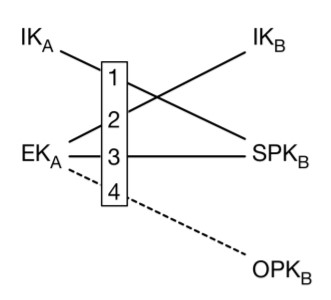
\includegraphics[width=0.4\linewidth]{images/X3dh}
	\caption{DH calculations.}
	\label{fig:x3dh}
\end{figure}
The DH outputs are fed into a key derivation function (KDF) to generate the shared secret $ SK $. Next, Alice deletes her $ EK_{A_{p}}$ and all DH outputs for forward secrecy. At this moment, Alice is ready to send the initial message with the content encrypted using $ SK $. The initial message from Alice to Bob has to have enough information for Bob to generate the same $ SK $.
The initial message contains:
\begin{itemize}\setlength\itemsep{-0.3em}
	\item $ IK_{A} $
	\item $ EK_{A} $
	\item Identifiers of Bob's prekeys used by Alice
	\item An initial ciphertext. The ciphertext can be used as an initial message for a post-X3DH communication protocol, e.g. Double ratchet algorithm.
\end{itemize}
\subsubsection{Bob's $ SK $ Derivation}
Using the key identifiers sent by Alice, Bob loads the private keys corresponding to the public keys Alice used. In combination with the keys $ IK_{A} $ and $ EK_{A} $ Alice sent, Bob can compute the same $ SK $ by doing the three (or four) DH operations.
\par
Next, Bob attempts to decrypt the ciphertext. If the message is successfully decrypted to the expected format, e.g. the format of the first message of the post-X3DH protocol, then the protocol run was successful. Otherwise, Bob aborts the protocol and discards the $ SK $.
\subsection{Security Considerations}
\subsubsection{Authentication}
Authentication is essential for both parties to guarantee the identity of who they are communicating with. Thus, Alice and Bob must authenticate the keys $ IK_{A} $ and $ IK_{B} $. The specification does not discuss authentication methods.
\subsubsection{Protocol Replay}
The one-time prekey used in the fourth and optional DH calculation is for protection against replay attacks as they ensure freshness of the protocol run. Absence of a one-time prekey could lead a replayed message to be accepted by Bob believing that Alice had sent it in the current protocol run.
\subsubsection{Server Trust}
A server can be a cause of attacks if malicious. It can carry out a Denial of Service attack if it refuses to forward the messages. It can deliberately not distribute one-time prekeys, exposing the protocol to replay attacks. Also, one party can drain all the one-time prekeys, if the server is not attentive to such action, leading to replay attacks.

\section{OFMC Modelling}
Presented in listing \ref{model} the code for modelling the protocol in OFMC using the language AnB. This section explains the code of the model section by section.
\lstinputlisting[numbers=left,                    
numberblanklines=false, breaklines=true, columns=fullflexible,
frame=single,
breaklines=true,
postbreak=\mbox{\textcolor{red}{$\hookrightarrow$}\space},
caption={X3DH OFMC Model},captionpos=b, label={model}]{code/x3dh.anb}

\subsection{Types section} 
Here, the parameters of the protocol are defined, e.g. variables, constants, roles, etc. Line 4 defines the participants of the protocol of type \textbf{Agent}.
\begin{itemize}\setlength\itemsep{-0.3em}
	\item A and B: Variables indicating Alice and Bob. A variable may be dishonest in an OFMC protocol run.
	\item s: Constant indicating the server. Constants act as trusted third parties.
\end{itemize}
\par
Line 5 defines the functions of the protocol.
\begin{itemize}\setlength\itemsep{-0.3em}
	\item kdf: Key derivation function.
	\item pk: A function to model asymmetric key pairs. A public key for Alice is modeled as pk(A) and the corresponding private key is computed using the internal function inv() as follows inv(pk(A)).
	\item ik: models the private component of the identity key of a party for the DH calculations.
\end{itemize}
	Alice and Bob have long-term signing keys modeled by the function `pk()` and long-term identity keys modeled by the function `ik()`.
	\par
Line 6 defines the numbers used in the protocol. Lower-case numbers are constants, while upper-case numbers are random and freshly generated during a protocol run. Some private components of keys are modeled as numbers as they are required to be freshly generated during a protocol run which can not be done using functions.
\begin{itemize}\setlength\itemsep{-0.3em}
	\item g: Public exponent base for DH calculations.
	\item NA: Alice's Nonce.
	\item EKA: The private component of Alice's Ephemeral key.
	\item OTP: The One-time prekey's private component.
	\item PREKEY: the prekey's private component.
	\item MSG1 and MSG2: Random numbers used as placeholders for random and fresh messages.
\end{itemize}

\subsection{Knowledge section}
This section of the model defines what knowledge is initially known to each party before the protocol starts. Line 9 defines Alice's knowledge which contains, in addition to the previously defined parameters, Alice's certificate modeled as `\{A, pk(A)\}inv(pk(s))`. This translates to Alice's identity `\textbf{A}` and Alice's public key `\textbf{pk(A)}` are signed using the servers private key `\textbf{inv(pk(s))}'. 

Line 15 holds a `where` clause that strictly defines A and B as different parties to avoid the scenario where A or B talk to itself.
\subsection{Actions section}
The Actions section states the protocol's message sequence between the participating parties for a successful protocol run. Throughout this section messages are referred to according to their line number, e.g message 19 is the message in line number 19 of the model code.
\par
Message 19 represents the registration phase where Bob publishes his public information to the server. The message contains the following:
\begin{itemize}\setlength\itemsep{-0.3em}
	\item exp(g,(XX)): The public DH key of the corresponding private key XX
	\item \{exp(g,PREKEY)\}inv(pk(B)): The prekey of Bob signed by Bob's signing key.
\end{itemize}
The whole message is encrypted for the server for authenticity.
\par
Message 21 is not an actual part of the protocol, however, it is included for the sake of modeling the protocol with the chosen tool. This is because of the asynchronous communication model of OFMC and the strands concept \cite{ofmcTut}.
\par 
In message 23, Alice requests to fetch from the server a key bundle to communicate with Bob. A nonce `NA` is attached for freshness.
\par
Message 25 is the server's response to Alice's key bundle request. The message contains the requested key bundle required to communicate with Bob, as well as Alice's nonce. The whole message is integrity protected by the server's signature.
\par
Message 27 represents the initial message from Alice to Bob. It is composed of the following:
\begin{itemize}\setlength\itemsep{-0.3em}
	\item Alice's certificate for authenticity.
	\item (Line 29) The Bob's keys which Alice will use to compute $ SK $. All these keys are signed by Alice for integrity protection.
	\item (Line 31) The initial ciphertext encrypted by the symmetric key $ SK $. The output of the 4 DH operations is input into the KDF resulting in $ SK $. 
\end{itemize}
\par
Message 38 is the last message of the protocol run. It is where Bob shows he is able to compute the same $ SK $. 
\subsection{Goals section}
This section of the model lists the security goals which the protocol must achieve at the end of a run. There are two types of goals
\begin{itemize}\setlength\itemsep{-0.3em}
	\item Authenticity: When a party wants to make sure a certain message has been generated and sent by the other party. In this model, Alice and Bob authenticate each others' public keys. Bob authenticates the server on the keys he received in message 27 from Alice, to be sure that the keys are forwarded by Alice from the server without tampering.
	\item Secrecy: The requirement for a message to be secret only between some parties.
\end{itemize}




\section{Difference from specification}
\subsection{Registration Phase}
The specification was not specific about how to securely publish Bob's keys to the server and the security of the connection between the server and the communicating parties. Therefore, the registration message from Bob to the server is encrypted by the server's public key.
\subsection{Use of Signatures}
The specification discouraged the use of signatures as they reduce deniability which is a desired feature in the messaging application setting which the protocol is intended for. However, this model used signatures.
\begin{enumerate}
	\item Signature are used in responses from the server to assure integrity of messages to receivers.
	\item Alice and Bob have an additional key pair for signing other than the identity key pairs. They are used to sign parts of messages which were vulnerable to attacks by intruders and would break the protocol's security. For example, Bob's keys which Alice used to compute $ SK $ in message 27.
\end{enumerate}
\subsection{Use of Certificates}
Alice used a certificate signed by the server to authenticate itself in-band as opposed to the specification which ruled the authentication between the parties as a necessary but out of scope operation.
\section{Conclusion}
\underline{\textbf{TODO: concluding paragraph}}
